\section{Timing: field, amplitude and walk}\label{app:timingdetails}
\intent{What the drift-field scan and the amplitude dependence say about the 40\,ns event time of chamber~A
(Dylan 2026-11-03: panel (c) of the timing figure moved here).}

On chamber~A at 490\,V (the 6-27 drift scan, reference-matched tracks), the event time falls from 114 to 79, 52, 41, 42
and 38\,ns as the drift field rises from 106 to 177, 248, 319, 355 and 390\,V/cm, and the uncorrelated part $(t_X-t_Y)/\sqrt2$
from 46 to 22\,ns (\cref{fig:timing_driftscan}). Three things follow.
(i) The time resolution is signal-to-noise, not walk. At a fixed HV it falls with the early amplitude of the track
(\crefp{fig:timing}{b}), and Runs 1 and 2 binned in that amplitude at one HV lie on the same curve as every scan row
(within 0.89--1.01 of it). A walk correction (the median time against amplitude) moves the event time of Runs 1 and 2 from 40.7 to
40.5\,ns and leaves the uncorrelated part at 22.3\,ns: across the amplitude quartiles the median moves by 18 and
3.7\,ns against widths of 41 and 22\,ns.
(ii) At fixed amplitude the HV barely matters: in a fixed early-amplitude window (1000--1600\,ADC) the event time is $44\pm5$\,ns at 435\,V
and $30\pm4$ at 490\,V (\cref{sec:efficiency}), consistent with a constant ($\chi^2/\mathrm{dof}=1.5$). The gain
sets where a track sits on the curve.
(iii) What does not fall is the part common to X and Y, ${\sim}38$\,ns at the top of the scan (the arrival of the first
electrons, read by both views). In drift distance, with each row's timing velocity (17.7 to 37.2\,\textmu m/ns), the event time
is $1.3$--$1.5$\,mm at every field from 177 to 390\,V/cm and the common part $1.2$--$1.4$\,mm (${\approx}1.3$\,mm), so
the floor is a depth, roughly constant in field, and the nanoseconds are that depth divided by a velocity that grows with the field.
The 106\,V/cm row has no distance (the column overruns the readout window, so no timing velocity was measured), and
the 100\,V/cm row has no matched clean trigger. The scan shows that the floor is a depth, and does not say where in the
chamber that depth comes from.
\begin{figure}[tbp]
  \centering
  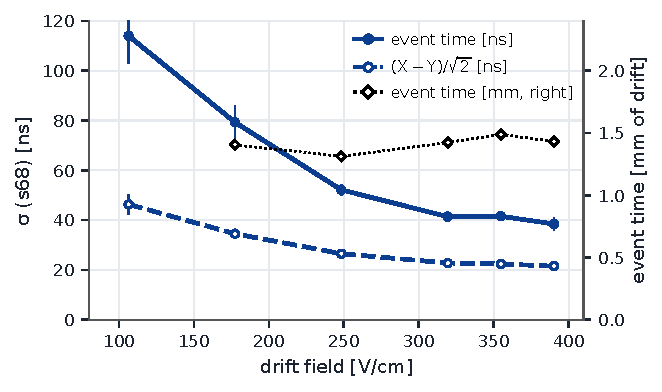
\includegraphics[width=0.7\linewidth]{timing_driftscan}
  \caption{Chamber~A time resolution against the drift field at 490\,V (M3-matched tracks, $s_{68}$): event time (solid) and $(t_X-t_Y)/\sqrt2$ (dashed) in ns, and, right axis, the event time in mm of drift (the row's timing velocity times the time; not available at 106\,V/cm). Error bars: statistical.}
  \label{fig:timing_driftscan}
\end{figure}
